% GNUPLOT: LaTeX picture with Postscript
\begingroup
  \makeatletter
  \providecommand\color[2][]{%
    \GenericError{(gnuplot) \space\space\space\@spaces}{%
      Package color not loaded in conjunction with
      terminal option `colourtext'%
    }{See the gnuplot documentation for explanation.%
    }{Either use 'blacktext' in gnuplot or load the package
      color.sty in LaTeX.}%
    \renewcommand\color[2][]{}%
  }%
  \providecommand\includegraphics[2][]{%
    \GenericError{(gnuplot) \space\space\space\@spaces}{%
      Package graphicx or graphics not loaded%
    }{See the gnuplot documentation for explanation.%
    }{The gnuplot epslatex terminal needs graphicx.sty or graphics.sty.}%
    \renewcommand\includegraphics[2][]{}%
  }%
  \providecommand\rotatebox[2]{#2}%
  \@ifundefined{ifGPcolor}{%
    \newif\ifGPcolor
    \GPcolortrue
  }{}%
  \@ifundefined{ifGPblacktext}{%
    \newif\ifGPblacktext
    \GPblacktexttrue
  }{}%
  % define a \g@addto@macro without @ in the name:
  \let\gplgaddtomacro\g@addto@macro
  % define empty templates for all commands taking text:
  \gdef\gplbacktext{}%
  \gdef\gplfronttext{}%
  \makeatother
  \ifGPblacktext
    % no textcolor at all
    \def\colorrgb#1{}%
    \def\colorgray#1{}%
  \else
    % gray or color?
    \ifGPcolor
      \def\colorrgb#1{\color[rgb]{#1}}%
      \def\colorgray#1{\color[gray]{#1}}%
      \expandafter\def\csname LTw\endcsname{\color{white}}%
      \expandafter\def\csname LTb\endcsname{\color{black}}%
      \expandafter\def\csname LTa\endcsname{\color{black}}%
      \expandafter\def\csname LT0\endcsname{\color[rgb]{1,0,0}}%
      \expandafter\def\csname LT1\endcsname{\color[rgb]{0,1,0}}%
      \expandafter\def\csname LT2\endcsname{\color[rgb]{0,0,1}}%
      \expandafter\def\csname LT3\endcsname{\color[rgb]{1,0,1}}%
      \expandafter\def\csname LT4\endcsname{\color[rgb]{0,1,1}}%
      \expandafter\def\csname LT5\endcsname{\color[rgb]{1,1,0}}%
      \expandafter\def\csname LT6\endcsname{\color[rgb]{0,0,0}}%
      \expandafter\def\csname LT7\endcsname{\color[rgb]{1,0.3,0}}%
      \expandafter\def\csname LT8\endcsname{\color[rgb]{0.5,0.5,0.5}}%
    \else
      % gray
      \def\colorrgb#1{\color{black}}%
      \def\colorgray#1{\color[gray]{#1}}%
      \expandafter\def\csname LTw\endcsname{\color{white}}%
      \expandafter\def\csname LTb\endcsname{\color{black}}%
      \expandafter\def\csname LTa\endcsname{\color{black}}%
      \expandafter\def\csname LT0\endcsname{\color{black}}%
      \expandafter\def\csname LT1\endcsname{\color{black}}%
      \expandafter\def\csname LT2\endcsname{\color{black}}%
      \expandafter\def\csname LT3\endcsname{\color{black}}%
      \expandafter\def\csname LT4\endcsname{\color{black}}%
      \expandafter\def\csname LT5\endcsname{\color{black}}%
      \expandafter\def\csname LT6\endcsname{\color{black}}%
      \expandafter\def\csname LT7\endcsname{\color{black}}%
      \expandafter\def\csname LT8\endcsname{\color{black}}%
    \fi
  \fi
    \setlength{\unitlength}{0.0500bp}%
    \ifx\gptboxheight\undefined%
      \newlength{\gptboxheight}%
      \newlength{\gptboxwidth}%
      \newsavebox{\gptboxtext}%
    \fi%
    \setlength{\fboxrule}{0.5pt}%
    \setlength{\fboxsep}{1pt}%
\begin{picture}(8786.00,5102.00)%
    \gplgaddtomacro\gplbacktext{%
      \csname LTb\endcsname%%
      \put(132,2991){\makebox(0,0)[r]{\strut{}$0$}}%
      \put(132,4644){\makebox(0,0)[r]{\strut{}$2$}}%
      \put(393,2815){\makebox(0,0){\strut{}$0.95$}}%
      \put(1854,2815){\makebox(0,0){\strut{}$1.1$}}%
      \put(2827,2815){\makebox(0,0){\strut{}$1.2$}}%
    }%
    \gplgaddtomacro\gplfronttext{%
      \csname LTb\endcsname%%
      \put(-11,3980){\rotatebox{-270}{\makebox(0,0){\small DBI [-]}}}%
      \put(3681,2771){\makebox(0,0){\large $\varepsilon$ {\small [\AA]}}}%
      \csname LTb\endcsname%%
      \put(706,3812){\makebox(0,0){\small k=7 \hskip 0.1cm}}%
      \csname LTb\endcsname%%
      \put(706,3636){\makebox(0,0){\small k=6 \hskip 0.1cm}}%
      \csname LTb\endcsname%%
      \put(706,3460){\makebox(0,0){\small k=5 \hskip 0.1cm}}%
      \csname LTb\endcsname%%
      \put(706,3284){\makebox(0,0){\small k=4 \hskip 0.1cm}}%
    }%
    \gplgaddtomacro\gplbacktext{%
      \csname LTb\endcsname%%
      \put(4525,2991){\makebox(0,0)[r]{\strut{}$0$}}%
      \put(4525,4809){\makebox(0,0)[r]{\strut{}$132$}}%
      \put(4797,2815){\makebox(0,0){\strut{}$0.95$}}%
      \put(6342,2815){\makebox(0,0){\strut{}$1.1$}}%
      \put(7373,2815){\makebox(0,0){\strut{}$1.2$}}%
      \put(4694,4437){\makebox(0,0)[l]{\strut{}\small optimal \textcolor{juliablue}{k=4}}}%
    }%
    \gplgaddtomacro\gplfronttext{%
      \csname LTb\endcsname%%
      \put(4382,3980){\rotatebox{-270}{\makebox(0,0){\strut{}\small pSF [-]}}}%
      \put(8184,2771){\makebox(0,0){\large $\varepsilon$ {\small [\AA]}}}%
    }%
    \gplgaddtomacro\gplbacktext{%
      \csname LTb\endcsname%%
      \put(132,440){\makebox(0,0)[r]{\strut{}0\%}}%
      \put(132,2507){\makebox(0,0)[r]{\strut{}100\%}}%
      \put(393,264){\makebox(0,0){\strut{}$0.95$}}%
      \put(1854,264){\makebox(0,0){\strut{}$1.1$}}%
      \put(2827,264){\makebox(0,0){\strut{}$1.2$}}%
      \put(1756,1680){\makebox(0,0)[l]{\strut{}\shortstack{\small\textcolor{black}{92 noise frames} \\ \small with \textcolor{juliablue}{k=4}}}}%
    }%
    \gplgaddtomacro\gplfronttext{%
      \csname LTb\endcsname%%
      \put(-11,1473){\rotatebox{-270}{\makebox(0,0){\strut{}\small Noise [\%]}}}%
      \put(3681,220){\makebox(0,0){\large $\varepsilon$ {\small [\AA]}}}%
    }%
    \gplgaddtomacro\gplbacktext{%
      \csname LTb\endcsname%%
      \put(4459,520){\makebox(0,0)[r]{\strut{}$13$}}%
      \put(4459,2291){\makebox(0,0)[r]{\strut{}$300$}}%
      \put(4797,264){\makebox(0,0){\strut{}$0.95$}}%
      \put(6342,264){\makebox(0,0){\strut{}$1.1$}}%
      \put(7373,264){\makebox(0,0){\strut{}$1.2$}}%
      \put(6548,1162){\makebox(0,0)[l]{\strut{}\shortstack{\small\textcolor{black}{13 clusters} \\ \small with \textcolor{juliablue}{k=4}}}}%
    }%
    \gplgaddtomacro\gplfronttext{%
      \csname LTb\endcsname%%
      \put(4382,1473){\rotatebox{-270}{\makebox(0,0){\strut{}\small Clusters [-]}}}%
      \put(8184,220){\makebox(0,0){\large $\varepsilon$ {\small [\AA]}}}%
    }%
    \gplbacktext
    \put(0,0){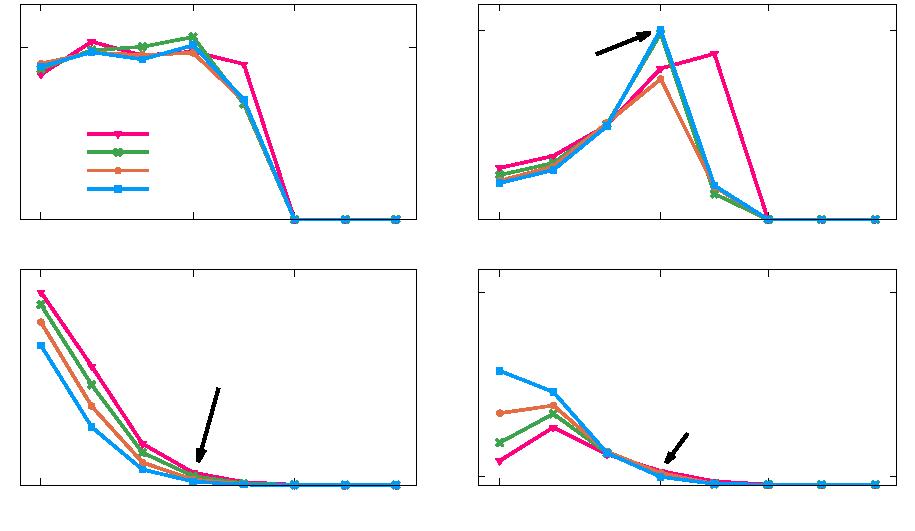
\includegraphics[width={439.30bp},height={255.10bp}]{../water_clustering_ca}}%
    \gplfronttext
  \end{picture}%
\endgroup
